\documentclass[UTF8]{ctexart}
\usepackage{graphicx}
\usepackage{float}
\usepackage{ragged2e}
\usepackage{amsthm}
\usepackage{tikz}
\usepackage{tikz-feynhand}
\usetikzlibrary{arrows.meta}
\newtheorem{problem}{题}
\newtheorem{solution}{解}
\usepackage{amssymb}
\usepackage{amsmath}
\usepackage{wrapfig}
\usepackage{hyperref}
\newcommand{\D}{\mathrm{d}}
\renewcommand\abstractname{须知} 
\title{题目}
\author{limbo137}
\begin{document}
\maketitle
\begin{abstract}
    在开始之前,我们需要熟悉一些物理学中常用但是你不一定非常了解的事情。对时间求导在物理上往往在函数上方打点,例如
    \[\frac{\D x}{\D t} = \dot{x}\]
    以及著名的Euler公式
    \[e^{i\theta} = \cos\theta + i\sin\theta\]
    还可以思考这个复数以及$\theta$在复平面上的意义
\end{abstract}
\[
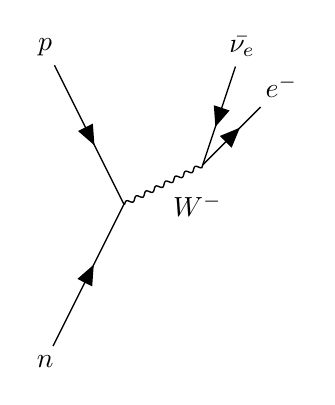
\begin{tikzpicture}
    \begin{feynhand}
        \vertex (a) at (0,0);
        \vertex (a1) at (-1,-2) {$n$};
        \vertex (a2) at (-1,2) {$p$};
        \vertex (b) at (1,0.5);
        \vertex (c1) at (1.5,2) {$\bar{\nu_e}$};
        \vertex (c2) at (2,1.5) {$e^-$};
        \node[below right] (B) at (0.5,0.25) {$W^-$};
        \propag[bos] (a) to (b);
        \propag[fer] (a1) to (a);
        \propag[fer] (a2) to (a);
        \propag[antfer] (b) to (c1);
        \propag[fer] (b) to (c2);
    \end{feynhand}
\end{tikzpicture}
\]
虚数$i$被物理学家Roger Penrose称为“魔数(The magic number)”,包含虚数在内的复数(complex number)在物理学中用处巨大,本题旨在用几个例子来初窥复数的奥秘。
\[i^2 = -1\]
\subsection{简谐振动}
经典力学中一类重要的运动称为简谐振动(simple harmonic vibration),这类运动往往有一个和坐标反向且成正比的力,于是其加速度也就和坐标反向且成正比,即
\begin{equation}
    a = -\omega^2 x \label{eq:a}
\end{equation}
其中$\omega^2$是比例系数。
我们知道,速度和加速度实际上是$x$的一阶导数和二阶导数,即
\begin{align*}
    v &= \frac{\D x}{\D t} \\
    a &= \frac{\D^2 x}{\D t^2} 
\end{align*}
1)求$x = e^{at}$的导数,以及二阶导数,试求出满足(\ref{eq:a})式的a值。\\
2)设$\omega u =v$,那么就有下面的方程组
\begin{equation}
\begin{split}
    \frac{\D x}{\D t}&= \omega u \\
    \frac{\D u}{\D t }&= -\omega x  \label{eq:b}
\end{split}
\end{equation}
试将该方程组写成矩阵形式。\\
3)找出这样的矩阵$A$满足
\[A^2 = -I\]
$I$为单位矩阵,与上面的矩阵形式相比较。\\
4)再设
\[r= x + iu\]
将(\ref{eq:b})写成$r$与$\frac{\D r}{\D t }$的关系。\\
5)当$t=0$时,$r=r_0 = A_0e^{i\phi}$,我们把$r_0$称为复振幅(complex amplitude)。
求解4)中的$r$,并在复平面上表示
\subsection{平面运动}
%\[i = \begin{bmatrix}0&1\\-1&0\end{bmatrix}\]
在研究平面运动时我们往往利用复数表示平面的坐标,即
\[(x,y) \rightarrow r = x+ iy\]
这样做的好处是在极坐标中
\begin{equation}
    (\rho,\theta) \rightarrow r = \rho e^{i\theta} \label{eq:pl}
\end{equation}
利用式(\ref{eq:pl})我们可以求出
\[\frac{\D r}{\D t } = \frac{\D \rho}{\D t}e^{i\theta}+i\rho e^{i\theta}\frac{\D \theta}{\D t}\]
为了方便,我们利用上方打点的写法
\begin{equation}
    v = \dot{r} = \dot{\rho}e^{i\theta}+i\rho \dot{\theta} e^{i\theta} \label{eq:plv}
\end{equation}
此时$e^{i\theta}$前的系数就是速度$v$沿位置矢量方向的分量,也叫径向分量,$ie^{i\theta}$是与径向垂直的分量,称为切向分量,对于上例我们就有
\begin{align*}
    v_r &=  \dot{\rho}\\
    v_\theta&=\rho \dot{\theta}
\end{align*}
仿照上面的过程(或利用极坐标的Christoffel符号),求加速度$a$的径向分量和切向分量
\subsection{电磁正交场}
在一个电场与磁场互相垂直的空间内,一带电荷量为$q$的粒子在某一垂直于磁场方向的平面内运动,初速度和电场方向夹角为$\theta_0$,大小为$v_0$,我们可以初步画出图形
\[
\begin{tikzpicture}
    \draw[->] (-2,1) -- (2,1); 
    \draw[->] (-2,0) -- (3,0); 
    \draw[->] (-2,-1) -- (2,-1); 
    \draw[->] (0,-2) -- (0,2);
    \node[above left] (A) at (2,1) {$E$};
    \node[below right] (B) at (3,0) {$x$};
    \node[above right] (C) at (0,2) {$y$};
    \node[below right] (O) at (0,0) {$O$};
    \fill (-1,0.5) circle (2pt);
    \fill (-1,-0.5) circle (2pt);
    \fill (1,0.5) circle (2pt);
    \fill (1,-0.5) circle (2pt);
    \node[above left] (A) at (-1,0.5) {$B$};
    \draw[->] (0,0) -- (30:1);
    \node[above left] (O) at (30:1) {$v_0$};
    \node[below right] (O) at (0.33,0.44) {$\theta_0$};
    \draw (0:0.3) arc [start angle=0, end angle=30, radius=0.3cm];
\end{tikzpicture}
\]
在这种体系下,粒子所受的电磁力(是一个复数)可以写成
\[F = qE - i qv B\]
1)设$\frac{E}{B}=u$,$\frac{qB}{m}=\omega_0$,列出粒子的受力方程,并试图求解$v$与$t$的关系

(提示:方程
\[\frac{\D y}{\D x } = a+by\]
的通解是
\[y = Ce^{bx}-\frac{a}{b}\]
其中$C$由初值条件决定)\\
2)当$v_0 = 0$时,设$\frac{u}{\omega_0} = R$,求位矢$r$,进而求出位置随时间变动的参数方程

提示:
\[\int Ce^{bx}-\frac{a}{b} \D x = \frac{Ce^{bx}}{b}-\frac{a}{b}x + C_1\]
\subsection{Kepler运动}
Kepler运动指受经典引力下的运动,假设中心天体的质量为$M$,$M$足够大以至于可以看作惯性参考系,复平面中的引力可以写成
\begin{equation}
    F= -\frac{GMm}{\rho^2}e^{i\theta} \label{eq:gra}
\end{equation}
1)利用$F=ma$求加速度$a$\\
由开普勒第二定律我们知道,行星与中心天体的连线在相同的时间扫过相同的面积,那么单位时间该连线扫过的面积是守恒的,即下面的量守恒
\[L = v_{\theta}\rho = {\rho^2 \dot{\theta}} = 2{\D S \over \D t}\]
还可以写成
\begin{equation}
    L = \rho^2 \dot{\theta}\label{eq:agm}
\end{equation}
2)利用(\ref{eq:gra})和(\ref{eq:agm}),证明下面的量守恒
\[iLv+GMe^{i\theta}\]
如果在实的向量平面上,这个守恒的矢量称为Runge-Lenz矢量\\
3)假设粒子初始距离中心天体$\rho_0$,速度为垂直与位置矢量的$v_0$(如下图)
\[
\begin{tikzpicture}
    \draw[->] (0,-2) -- (0,2);
    \draw[->] (-2,0) -- (3,0);
    \node[below right] (B) at (3,0) {$x$};
    \node[above right] (C) at (0,2) {$y$};
    \node[below right] (O) at (0,0) {$M$};
    \fill (0,0) circle (2pt);
    \fill (2.1,0) circle (2pt);
    \draw[->] (2.1,0) -- (2.1,1.3);
    \node[below right] (B) at (2.1,1.3) {$v_0$};
    \node[below right] (B) at (1,0) {$\rho_0$};
\end{tikzpicture}
\]
求$v$复数随位移辐角$\theta$的变化,并将其画在以$\theta$为辐角的复平面上\\
4)利用上面的结果以及(\ref{eq:plv}),求在极坐标下该粒子运动的轨迹方程$\rho(\theta)$
\end{document}